\chapter{Entwicklung des Track-Cleaners}
In den vorangegangenen Kapiteln wurde auf die Grundlagen eingegangen, sodass in diesem Kapitel die Entwicklung des Track-Cleaners thematisiert werden kann. Dazu wurden zunächst die Problematiken genau analysiert um festzustellen, welche Eigenschaften der Track-Cleaner aufweisen muss. Ausgehend von der Aufgabenanalyse wurde dann ein Programmdesign erstellt, welches schließlich in C++ implementiert und in PandaRoot integriert wurde.

\section{Aufgabenanalyse}
Im Folgenden werden die unterschiedlichen Anforderungen an den Track-Cleaner kategorisiert und genauer analysiert.

\subsection{Unabhängigkeit von Detektor und Fitting-Algorithmus}
Der Track-Cleaner soll unabhängig vom konkreten Detektor, Fitting- oder Trackfinding-Algorithmus universell einsetzbar sein. Zum einen muss der Algorithmus in der Lage sein, einen Refit auszuführen, nachdem ein Hit aussortiert wurde. Teilchenflugbahnen, welche vom STT rekonstruiert werden, verwenden dazu einen Riemann-Fit. Dieser approximiert zu einer gegebenen Menge an Punkten die Kreisparameter genau so, dass der Abstand der Punkte von der Kreisbahn minimal wird. Prinzipiell sind jedoch auch andere Approximationen denkbar. Beispielsweise könnte eine Gerade als Fit benutzt werden, wenn die Flugbahn des Teilchens nicht von einem Magnetfeld beeinflusst wird. Der Fitting-Algorithmus muss folglich so gekapselt werden, dass er austauschbar ist ohne das Änderungen am Track-Cleaner nötig sind. Zum anderen wird eine Funktionalität benötigt, welche den minimalen Abstand eines Teilchens zum Fit berechnet. Die konkrete Implementierung ist also abhängig davon, welcher Fit bei der vorliegenden Teilchenflugbahn zu Grunde gelegt wird. In diesem Fall muss also ebenfalls die Schnittstelle von der Implementierung getrennt werden. Des Weiteren müssen die verwendeten Hits in einem vom konkreten Detektor unabhängigen Datentyp vorliegen und die Position des Hits beinhalten.

\subsection{Integrierbarkeit in PandaRoot}
Um den implementierten Algorithmus in PandaRoot integrieren zu können, müssen die von PandaRoot vorgegebenen Schnittstellen beachtet werden. Dazu existiert die abstrakte Klasse \code{FairTask}, welche über das objektorientierte Mittel der Vererbung derart erweiterbar ist, dass eigener Code ins Panda-Framework eingefügt werden kann. Dazu stellt die Oberklasse FairTask einige abstrakte Schnittstellen bereit, welche in der eigenen Klasse überschrieben werden müssen. Die Methode \code{InitStatus InitTask()} wird beim Start des Algorithmus einmal aufgerufen. Hier sollte in der eigenen Unterklasse eine Implementierung angegeben werden, welche unter anderem die benötigten Datenstrukturen initialisiert. Über den InitStatus muss zurückgegeben werden, ob die Initialisierungen erfolgreich waren. Danach wird für jedes Event einmal die Methode \code{void Exec(Option* opt)} ausgeführt, in welcher das eigentliche Verfahren implementiert werden muss. Im Anschluss daran wird für jedes Event die Methode \code{FinishEvent()} aufgerufen. Dies dient dazu, die verwendeten Datenstrukturen zurückzusetzen, sodass ein neues Event verarbeitet werden kann. Abschließend wird die Methode \code{Finish()} dazu verwendet, den allokierten dynamischen Speicher wieder freizugeben. Ein eigener FairTask kann dann in einem Root-Macro erstellt und dem FairRootManager zur Ausführung übergeben werden. Bei dem FairRootManager handelt es sich um eine Klasse, welche die Ausführung der verschiedenen FairTasks koordiniert und zum Zugriff auf Root-Branches verwendet werden kann.

\subsection{Ausführungsgeschwindigkeit}
Beim Rekonstruktionsverfahren des \pnd{}-Detektors handelt es sich um einen sogenannten Online-Tracker. Dies bedeutet, dass die Aufarbeitung der gemessenen Daten während der Durchführung des Experiments durchgeführt wird. Dies hat den Hintergrund, dass der \pnd{}-Detektor eine Datenmenge von 200
GB/s erzeugt. Eine Speicherung der entstehenden Daten ist mit der verfügbaren Speicherkapazität nicht möglich. Folglich müssen die Daten schon während des Experiments derart gefiltert werden, dass die Datengröße deutlich reduziert werden kann.

\subsection{Einfache Variation des Grenzwerts}
Im Rahmen dieser Arbeit soll auch erprobt werden, wie der vom Track-Cleaner verwendete Grenzwert am sinnvollsten zu wählen ist. Da sich dies am besten empirisch untersuchen lässt, ist es sinnvoll, den Track-Cleaner mit verschiedenen Grenzwerten zu testen und dann mittels eines Analyse-Macros die Qualität zu untersuchen. Dazu wurde ein externes Skript entwickelt, welches zu angegebener Startdistanz, Schrittweite und Enddistanz zuerst das Rekonstruktions-Macro und dann das Analyse-Macro aufruft. Folglich ist es nötig, das Verfahren derart zu parametrisieren, dass der verwendete Grenzwert ohne Mehraufwand beim Starten der Macros übergeben werden kann. Im Anschluss daran müssen die aus der Analyse gewonnenen Daten geeignet dargestellt werden, um eine angenehme Auswertung möglich zu machen.

\subsection{Problematik der gedrehten Straw-Tubes}
Unabhängig von der Höhe, in der eine normale Straw-Tube von einem Teilchen getroffen wurde ergibt sich in der 2-dimensionalen Projektion immer der gleiche Punkt. Dies ist bei gedrehten Straw-Tubes nicht der Fall, da die 2-Dimensionale Projektion der Tube keinen Punkt sondern eine Strecke liefert. Erzeugt eine gedrehte Straw-Tube einen Hit, so wird dazu immer die mittlere Höhe der Straw-Tube als Position benutzt. In der Projektion liegt der Hit folglich nur dann auf dem Track, wenn das verursachende Teilchen die gedrehte Straw-Tube in der Mitte getroffen hat. Wird der Detektor weiter oben oder unten durchquert liegen die Hits der gedrehten Straw-Tubes sehr weit von dem Track entfernt. Folglich ist es nicht sinnvoll gedrehte Straw-Tubes in das Bereinigen mit einzubeziehen, da diese aufgrund des großen Abstands zum Track fehlerhaft entfernt werden würden.

\section{Programmentwurf}

\begin{figure}
  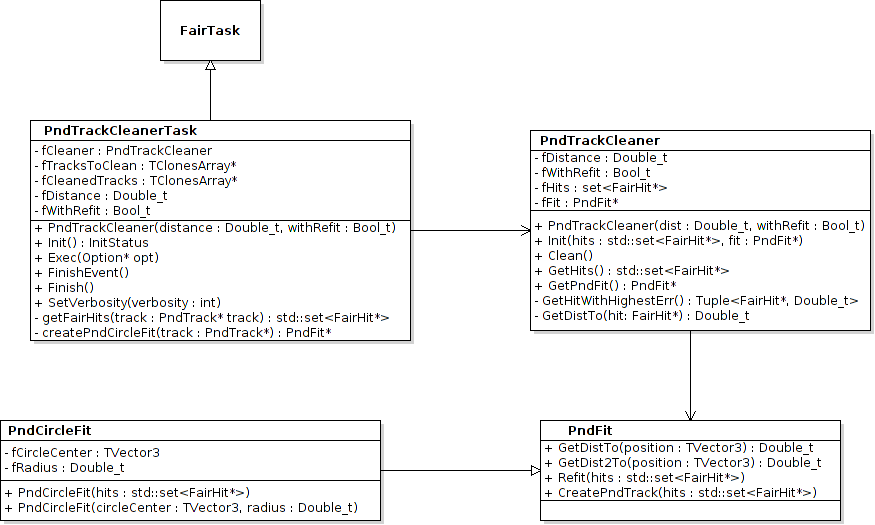
\includegraphics[width=0.9\textwidth]{Bilder/CleanerUML}
	\label{fig:CleanerUML}
	\caption{Veranschaulichung des Entwurfs mittels eines UML-Diagramm}
	
\end{figure}
Der Track-Cleaner wurde nach objektorientierten Grundsätzen entworfen. In Abbildung \ref{fig:CleanerUML} ist ein UML-Diagramm dargestellt, welches den Entwurf verdeutlicht. Es wurde eine Klasse \code{PndTrackCleanerTask} entwickelt, welche den oben erläuterten Vorgaben für eine FairTask genügt. Diese Klasse regelt den Dateizugriff und stellt das Bindeglied zwischen PandaRoot und dem eigentlichen Track-Cleaner dar. Die Klasse \code{PndFit} dient als abstrakte Schnittstelle für eine approximierte Teilchenflugbahn. Diese Schnittstelle umfasst im Wesentlichen die drei Methoden \code{GetDistTo)}, \code{Refit} und \code{CreatePndTrack}. Der Track-Cleaner hält einen Zeiger auf ein Objekt der Klasse PndFit und greift über diese Schnittstelle auf die zum Reinigen der Tracks benötigten Methoden zu. Im konkreten Fall von STT-Hits wird dazu die Unterklasse \code{PndCircleFit} benutzt. Diese legt einen Kreisfit als Approximation zu Grunde und benutzt einen Riemann-Fit um die Kreisparameter zu erzeugen. Der \code{PndTrackCleaner} arbeitet jedoch stets auf der Schnittstelle PndFit, sodass der konkrete Fitting-Algorithmus problemlos ausgetauscht werden kann. Damit es möglich ist, den verwendete Grenzwert \code{fDistance} über ein Skript zu variieren, kann dieser dem PndTrackCleanerTask im Konstruktor übergeben werden. Der Task kann somit den TrackCleaner mit dem übergebenen Wert initialisieren. Dies macht es möglich das ebenfalls parametrisierbare Rekonstruktions-Macro automatisiert mit verschiedenen Grenzwerten aufzurufen. Außerdem wurde ein weiteres Macro implementiert, welches alle Hit von gedrehten Straw-Tubes im Vorfeld aussortiert und einen neuen Root-Branch mit den Namen TracksToClean anlegt. Dieser Branch soll dem TrackCleaner als Eingabe dienen.

\section{Implementation des Verfahrens}
Da der Projektentwurf nun thematisiert wurde, folgen nun Erläuterungen zu den wichtigsten implementierten Methoden.

\subsection{PndTrackCleanerTask}
\begin{description}
	\item[InitStatus Init()] Diese Methode initialisiert zunächst den PndTrackCleaner mit dem Grenzwert fDistance und gibt an ob nach jedem herausgefilterten Punkt ein Refit durchgeführt werden soll. Im Anschluss daran wird der FairRootManager fIoman initialisiert. Dabei handelt es sich um ein Singelton, welches verwendet werden kann, um auf Root-Dateien zugreifen zu können. Danach wird der FairRootManager verwendet um die beiden \code{TClonesArray*} fCleanedTracks und fTracksToClean zu initialisieren. Diese beiden Objekte stellen den Zugriff auf die gleichnamigen Root-Branches her. TracksToClean wird dabei von einem Trackfinder erzeugt und beinhaltet die rekonstruierten Tracks. Der Branch CleanedTracks wird in der Init-Methode neu erstellt und wird mit den bereinigten Tracks gefüllt.
	
	\item[void Exec(Option\_t* opt)] Diese Methode extrahiert die benötigten Tracks aus einem Event und wandelt diese in ein Objekt der Klasse PndFit um. Außerdem werden die zum Cleanen benötigten FairHits von dem Track abgefragt. Mit diesen Daten wird daraufhin der eigentliche Cleaner initialisiert und gestartet. Im Anschluss daran werden die bereinigten Tracks in den neuen Branch CleanedTracks der Root-Datei geschrieben.
	
	\item[void FinishEvent()] Zu Beginn jedes Events werden die Objekte der Klasse TClonesArray* automatisch mit den Daten aus der Root-Datei befüllt. Damit diese beim nächsten Event keine ungültigen Daten mehr enthalten, werden sie in dieser Methode geleert.
	
	\item[void SetVerbosity(int verbosity)] Über diese Methode kann angegeben werden, welche Logging-Informationen bei der Ausführung des TrackCleaners ausgegeben werden sollen. Dabei werden die folgenden Klassifizierungen verwendet:
	\begin{enumerate}
		\item[verbosity=0] Keine Ausgabe
		\item[verbosity=1] Nur Fehler (Default)
		\item[verbosity=2] Fehler und wichtige Logging-Informationen
		\item[verbosity=3] Detailierte Ausgabe, sodass die Programmfunktionalität genau nachvollzogen werden kann.
	\end{enumerate}
	
	\item[std::set<FairHit*> getFairHits(PndTrack* track)] Diese Methode extrahiert aus dem übergebenen PndTrack die Menge an FairHits, welche dem Track zugeordnet worden ist.
	
	\item[PndFit* createPndCircleFit(PndTrack* track)] Um den TrackCleaner zu initialisieren, wird ein Objekt der Klasse PndFit benötigt. In dieser Methode wird dazu ein Objekt der Klasse PndCircleFit erstellt, welches die Teilchenflugbahn des übergebenen Tracks approximiert.
\end{description}

\subsection{PndTrackCleaner}
\begin{description}
	\item[void Clean()] Diese Methode führt die eigentliche Bereinigung des Tracks durch. Dazu wird in einer Schleife die private Methode GetHitWithHighestErr aufgerufen und überprüft, ob der minimale Abstand des zurückgegebenen Hits vom approximierten Track größer ist als zugelassene Grenzwert. Ist dies der Fall wird der gefundene Hit entfernt, evtl. ein Refit ausgeführt und das Verfahren dann wiederholt. Falls der Grenzwert nicht überschritten wird, kann das Verfahren hier abgebrochen werden.
	
	\item[Tuple<FairHit*, Double\_t> GetHitWithHighestErr()] In dieser Methode wird für jeden Hit der minimalen Abstand zum approximierten Track berechnet und der Hit ausgewählt, bei dem dieser Abstand am größten ist. Danach wird ein Tupel zurückgegeben, welches den ausgewählten Hit und den Abstand zum Track enthält.
	
	\item[Double\_t GetDistTo(FairHit* hit)] Diese Methode bestimmt den Abstand eines FairHits vom aktuellen Fit. Dazu wird auf die Methide PndFit::GetDist2To zurückgegriffen.
	
	\item[std::set<FairHit*> GetHits()] Nachdem das Reinigen eines Tracks abgeschlossen ist, wird der bereinigte Track vom PndTrackCleanerTask wieder in die Root-Datei geschrieben. Da dazu die verbleibenden Hits benötigt werden, können diese über die Methode GetHits abgefragt werden.
\end{description}

\subsection{PndCircleFit}
\begin{description}
	\item[Double\_t getDistTo(TVector3 position)] In dieser Methode wird zunächst der Abstandsvektor des übergebenen Punktes vom Kreismittelpunkt berechnet. Im Anschluss daran wird von der Norm dieses Vektors der Kreisradius subtrahiert um somit den Abstand des Punktes von der Kreisbahn zu berechnen. Da es sich beim Kreisfit um eine Projektion in die Ebene handelt, wird vor der Berechnung die z-Komponente des übergebenen Vektors auf 0 gesetzt.


	\item[void Refit(std::set<FairHit*> hits)] Nachdem ein Hit aus dem aktuellen Track entfernt wurde, muss gegebenenfalls ein Refit ausgeführt werden. Dazu wird in dieser Methode die Klasse PndRiemannFit benutzt um die Kreisparameter ausgehend von den übergebenen Hits anzupassen.

	\item[PndTrack CreatePndTrack(std::set<FairHit*> hits)] In dieser Methode wird ausgehend von den übergebenen Hits ein PndTrack erstellt, sodass dieser in der Root-Datei gespeichert werden kann. Dazu wird die Methode getPndTrack der Klasse PndRiemannTrack verwendet.
\end{description}